\documentclass[11pt]{report}

% Paquetes y configuraciones adicionales
\usepackage{graphicx}
\usepackage[export]{adjustbox}
\usepackage{caption}
\usepackage{float}
\usepackage{titlesec}
\usepackage{geometry}
\usepackage[hidelinks]{hyperref}
\usepackage{titling}
\usepackage{titlesec}
\usepackage{parskip}
\usepackage{wasysym}
\usepackage{tikzsymbols}
\usepackage{fancyvrb}
\usepackage{xurl}
\usepackage{hyperref}
\usepackage[spanish]{babel}
\usepackage{listings}
\usepackage{subcaption}
\usepackage{xcolor}
\usepackage{amssymb}

\newcommand{\subtitle}[1]{
  \posttitle{
    \par\end{center}
    \begin{center}\large#1\end{center}
    \vskip0.5em}
}

% Configura los márgenes
\geometry{
  left=2cm,   % Ajusta este valor al margen izquierdo deseado
  right=2cm,  % Ajusta este valor al margen derecho deseado
  top=3cm,
  bottom=3cm,
}

% Configuración de los títulos de las secciones
\titlespacing{\section}{0pt}{\parskip}{\parskip}
\titlespacing{\subsection}{0pt}{\parskip}{\parskip}
\titlespacing{\subsubsection}{0pt}{\parskip}{\parskip}

% Redefinir el formato de los capítulos y añadir un punto después del número
\makeatletter
\renewcommand{\@makechapterhead}[1]{%
  \vspace*{0\p@} % Ajusta este valor para el espaciado deseado antes del título del capítulo
  {\parindent \z@ \raggedright \normalfont
    \ifnum \c@secnumdepth >\m@ne
        \huge\bfseries \thechapter.\ % Añade un punto después del número
    \fi
    \interlinepenalty\@M
    #1\par\nobreak
    \vspace{10pt} % Ajusta este valor para el espacio deseado después del título del capítulo
  }}
\makeatother

% Configura para que cada \chapter no comience en una pagina nueva
\makeatletter
\renewcommand\chapter{\@startsection{chapter}{0}{\z@}%
    {-3.5ex \@plus -1ex \@minus -.2ex}%
    {2.3ex \@plus.2ex}%
    {\normalfont\Large\bfseries}}
\makeatother

% Configurar los colores para el código
\definecolor{codegreen}{rgb}{0,0.6,0}
\definecolor{codegray}{rgb}{0.5,0.5,0.5}
\definecolor{codepurple}{rgb}{0.58,0,0.82}
\definecolor{backcolour}{rgb}{0.95,0.95,0.92}

% Configurar el estilo para el código
\lstdefinestyle{mystyle}{
  backgroundcolor=\color{backcolour},   
  commentstyle=\color{codegreen},
  keywordstyle=\color{magenta},
  numberstyle=\tiny\color{codegray},
  stringstyle=\color{codepurple},
  basicstyle=\ttfamily\footnotesize,
  breakatwhitespace=false,         
  breaklines=true,                 
  captionpos=b,                    
  keepspaces=true,                 
  numbers=left,                    
  numbersep=5pt,                  
  showspaces=false,                
  showstringspaces=false,
  showtabs=false,                  
  tabsize=2
}

\begin{document}

\title{CANARY ISLANDS DATABASE}
\author{Samuel Martín Morales  \texttt{alu0101359526@ull.edu.es} \and Jorge Domínguez González  \texttt{alu0101330600@ull.edu.es} \and Cheuk Kelly Ng Pante \texttt{alu0101364544@ull.edu.es} }
\date{\today}

\maketitle

\chapter{Objetivos del Proyecto}
El objetivo del proyecto es el diseño, creación e implementación de una base de datos para gestionar información relacionada con las Islas Canarias.
La base de datos debe permitir realizar operaciones CRUD sobre la información almacenada en ella, así como consultas de prueba para demostrar su funcionamiento.


\chapter{Descripción del contexto de la base de datos}
La base de datos está destinada para almacenar información sobre las Islas Canarias, como por ejemplo, información sobre las islas, su distribución poblacional, compañías, sitios de interés y animales autóctonos.
La gestión de la información de las Islas Canarias es de gran importancia para el turismo, ya que permite a los turistas conocer mejor las islas y su historia, así como los lugares de interés que pueden visitar
y los animales o plantas autóctonas que se pueden encontrar en nuestro archipiélago.

\section{Entidades:}
\begin{itemize}
      \item \textbf{Isla:}
            \subitem - Atributos: ID (clave primaria), Nombre.

      \item \textbf{Distribución Poblacional:}
            \subitem - Atributos: ID (clave primaria), Nombre, Provincia, Capital, Municipio, Poblacion Isla.

      \item \textbf{Compañías:}
            \subitem - Atributos: ID (clave primaria), Nombre, Tipo, Sede (relacionada con Islas), Año Fundacion.

      \item \textbf{Comestibles:}
            \subitem - Atributos: ID (clave primaria), Nombre, Tipo, Compañia.

      \item \textbf{Productos:}
            \subitem - Atributos: ID (clave primaria), Nombre, Islas.

      \item \textbf{Artesania:}
            \subitem - Atributos: ID (clave primaria), Nombre, Creador, Tipo.

      \item \textbf{Sitio interes:}
            \subitem - Atributos: ID (clave primaria), Nombre, Islas, Nombre Isla, Municipio, Latitud, Longitud,

      \item \textbf{Folklore:}
            \subitem - Atributos: ID (clave primaria), Nombre, Lanzamiento, Autor.

      \item \textbf{Seres Vivos:}
            \subitem - Atributos: ID (clave primaria), Nombre.

      \item \textbf{Animales autóctonos:}
            \subitem - Atributos: ID (clave primaria), Nombre, Nombre Cientifico, Islas, Invasoras, Dieta.

      \item \textbf{Plantas autóctonas:}
            \subitem - Atributos: ID (clave primaria), Nombre, Nombre Cientifico, Islas, Invasoras.

      \item \textbf{Nombres Canarios:}
            \subitem - Atributos: ID (clave primaria), Nombre, Isla, Genero.

      \item \textbf{Platos:}
            \subitem - Atributos: ID (clave primaria), Nombre, Tipo.

      \item \textbf{Ingredientes:}
            \subitem - Atributos: ID (clave primaria), Nombre.
\end{itemize}

Entre estas entidades nos encontramos con los siguientes tipos de entidades:
\begin{itemize}
      \item \textbf{Entidades Fuertes:} Isla, Compañia, Comestibles, Productos, Artesania, Seres Vivos, Nombres Canarios, Platos, Ingredientes.
      \item \textbf{Entidades Débiles:} Distribución Poblacional, Sitio interes, Folklore, Animales autóctonos, Plantas autóctonas.
\end{itemize}

\section{Relaciones:}
Las relaciones entre las entidades son las siguientes:
\begin{itemize}
      \item \textbf{Isla a Distribución Poblacional}
            \subitem - Relacionada por la columna Nombre con la entidad Islas.

      \item \textbf{Compañías a Islas:}
            \subitem - Relacionada por la columna Sede con la entidad Islas.

      \item \textbf{Sitio interes a Islas:}
            \subitem - Relacionada por la columna Isla con la entidad Islas.

      \item \textbf{Animales autóctonos a Islas:}
            \subitem - Relacionada por la columna Islas con la entidad Islas.
\end{itemize}

\section{Consideraciones Adicionales:}

\begin{itemize}
      \item La relación entre las entidades Compañías y Islas se establece a través de la columna Sede, indicando la isla donde tienen su sede las compañías.
      \item La relación entre Sitios Interes y Islas se establece por la columna Isla, indicando en qué isla se encuentra el sitio de interés.
      \item La relación entre Animales autóctonos e Islas se establece por la columna Islas, indicando las islas a las que están asociados los animales autóctonos.
\end{itemize}

\section{Restricciones:}

\begin{itemize}
      \item La relación entre las entidades Compañías y Islas se establece a través de la columna Sede, indicando la isla donde tienen su sede las compañías.
      \item La relación entre Sitio interes y Islas se establece por la columna Isla, indicando en qué isla se encuentra el sitio de interés.
      \item La relación entre Animales autóctonos e Islas se establece por la columna Islas, indicando las islas a las que están asociados los animales autóctonos.
\end{itemize}
\chapter{Diseño Conceptual}

\section{Modelo Entidad-Relación}
\begin{figure}[H]
      \centering
      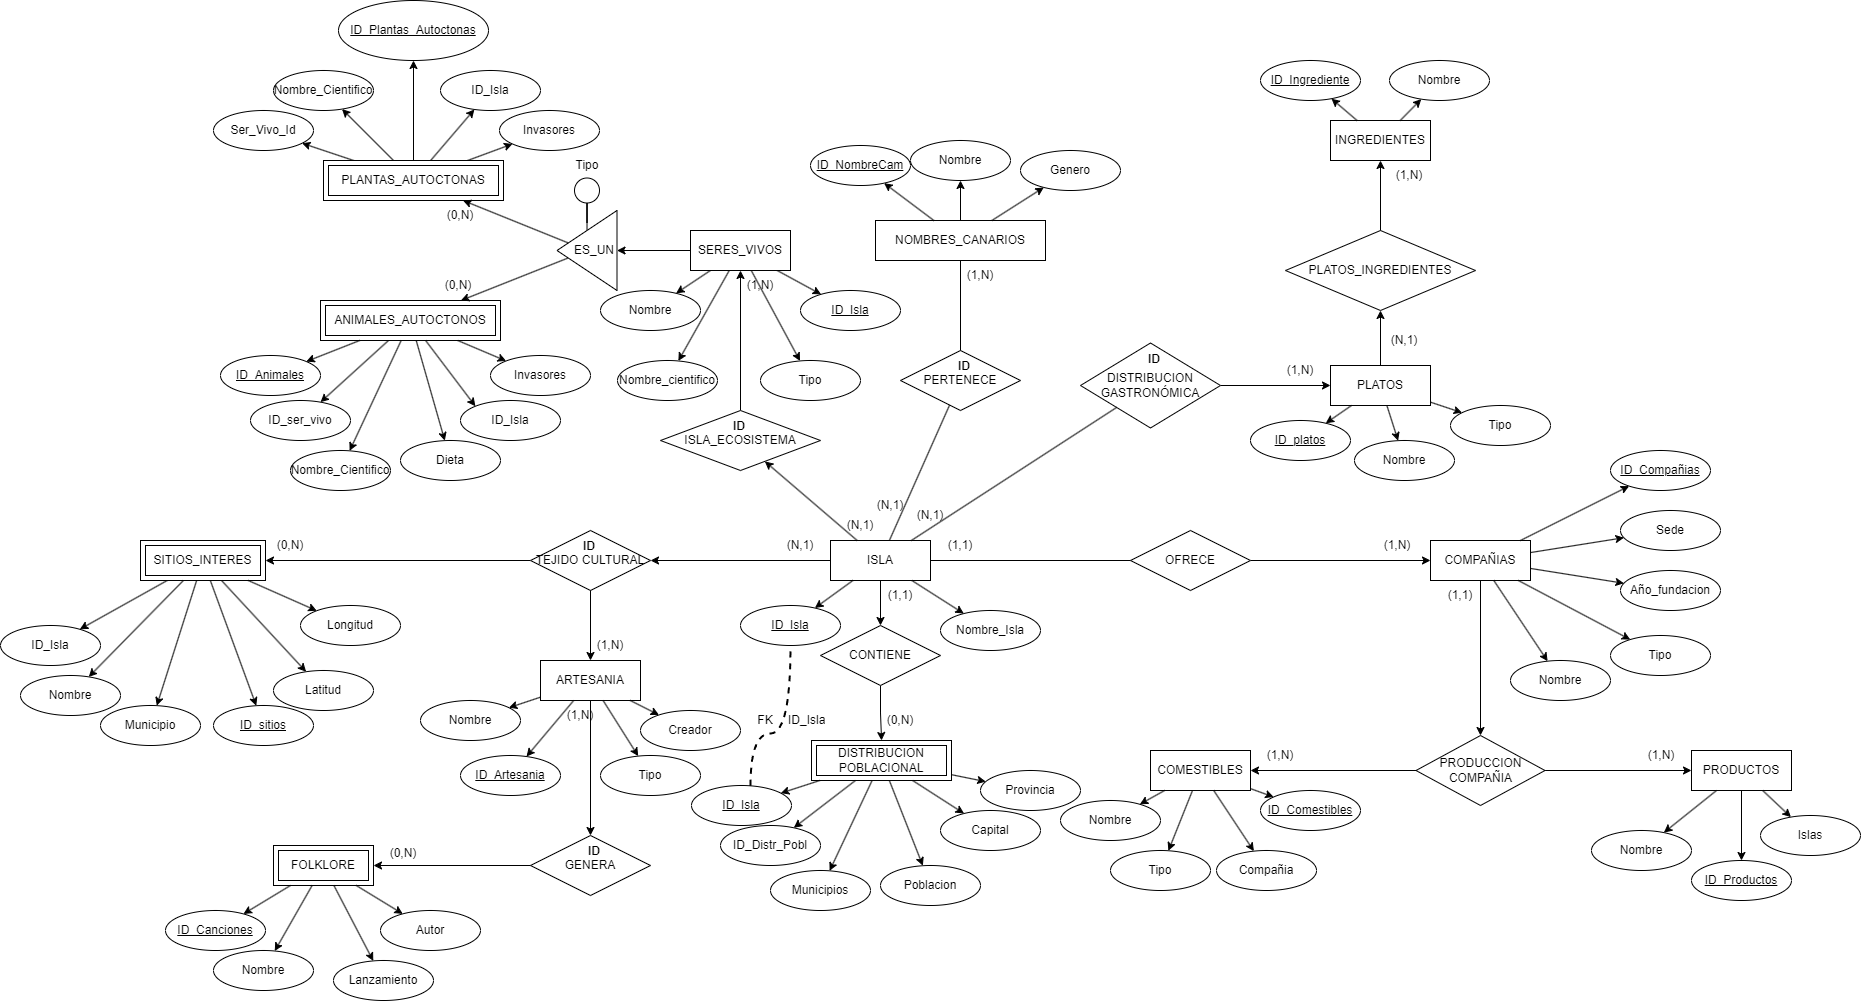
\includegraphics[width=0.9\textwidth]{../diagrams/ER-PF-ADBD.png}
      \caption{Modelo Entidad-Relación}
      \label{fig:modelo_er}
\end{figure}

\section{Modelo Relacional}
\begin{figure}[H]
      \centering
      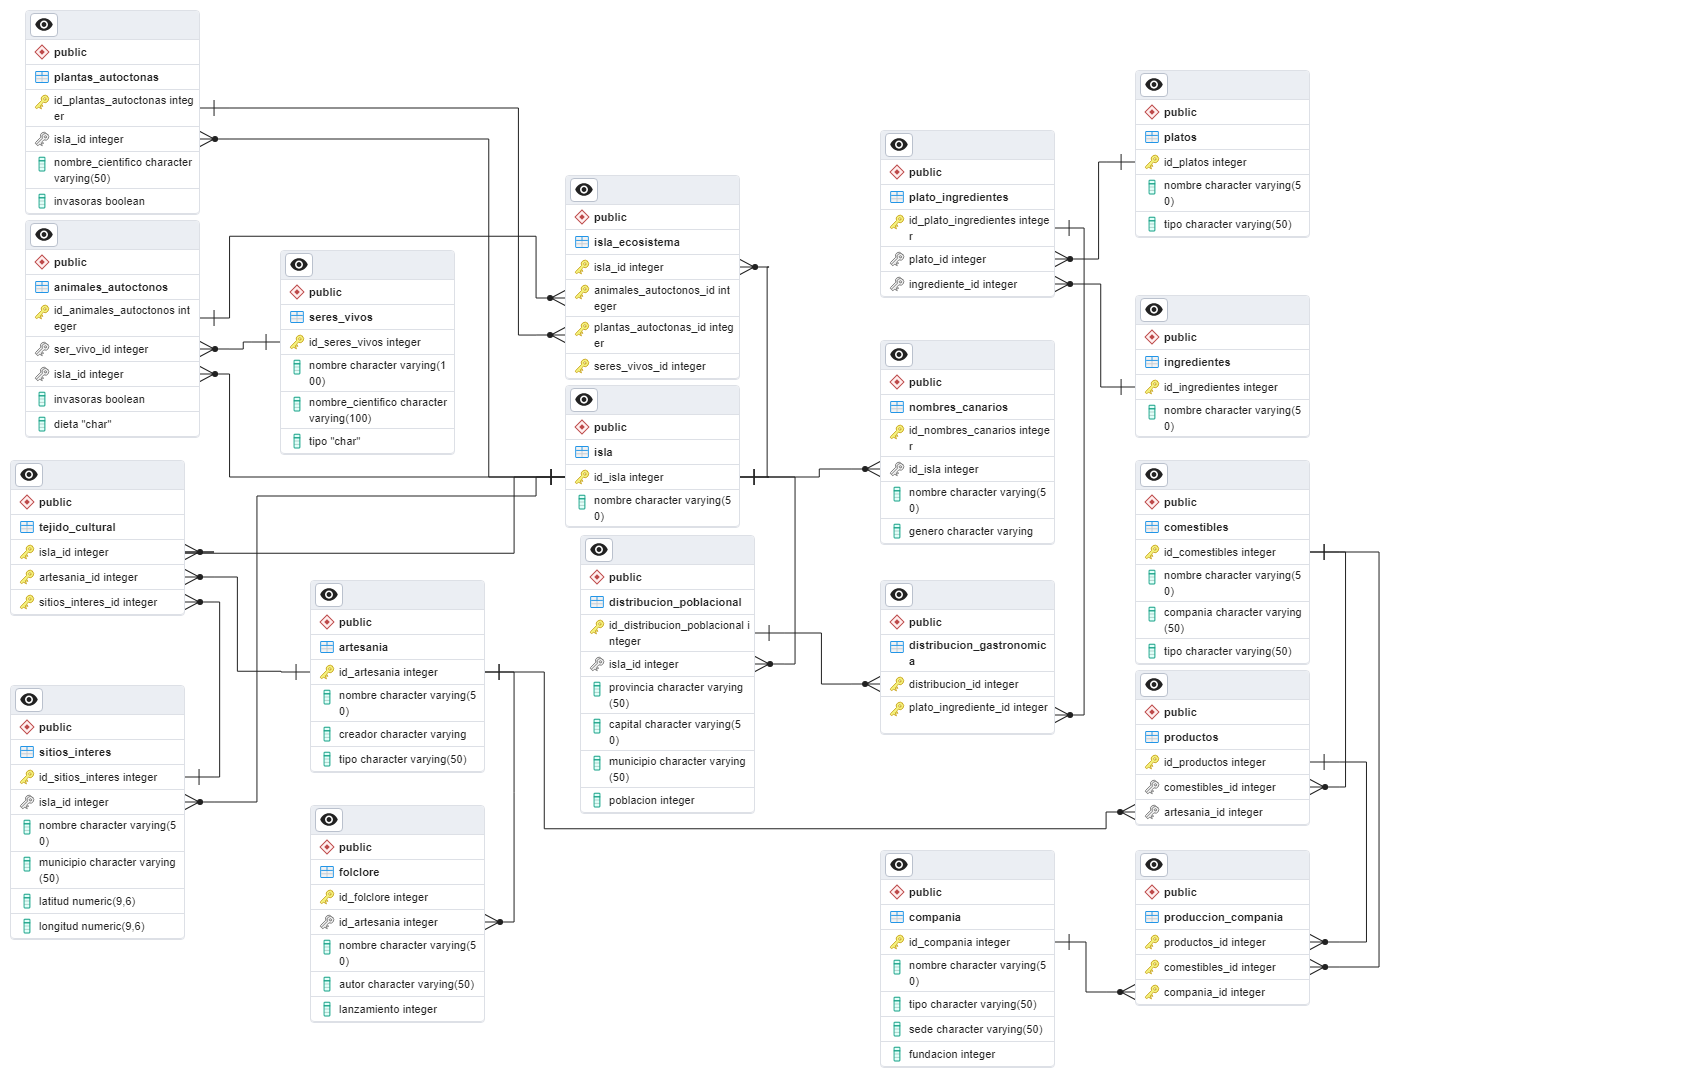
\includegraphics[width=0.9\textwidth]{../diagrams/RELACIONAL.png}
      \caption{Modelo Relacional}
      \label{fig:modelo_relacional}
\end{figure}

\section{Supuestos Semánticos}
Documentación que explique los supuestos semánticos y decisiones de diseño.

\chapter{Scripts SQL}
El script \emph{canary\_islands.sql} contiene la implementación de la base de datos en PostgreSQL. Para la ejecución
del script desde \emph{psql} se debe ejecutar el siguiente comando:
\begin{verbatim}
$ sudo -u postgres psql
postgres=# \i canary_islands.sql
\end{verbatim}

% Nueva pagina
\newpage

\section{Creación de la Base de Datos}
\lstset{style=mystyle}
\lstinputlisting[language=sql]{src/creation_db.sql}

\section{Inicialización de las tablas}
Al ejecutar el script \emph{canary\_islands.sql} se crean las tablas de la base de datos, así como las relaciones entre ellas.
\begin{itemize}
      \item \textbf{Tabla Isla:} Es una tabla que representa cada isla del archipiélago canario.
            \lstset{style=mystyle}
            \lstinputlisting[language=sql]{src/tables/table_isla.sql}

      \item \textbf{Tabla Seres Vivos:} Es una tabla que representa a los seres vivos que habitan en las islas.
            \lstset{style=mystyle}
            \lstinputlisting[language=sql]{src/tables/table_seres_vivos.sql}

      \item \textbf{Tabla Animales Autoctonos:} Es una tabla que contiene información sobre los animales autóctonos de las islas.
            \lstset{style=mystyle}
            \lstinputlisting[language=sql]{src/tables/table_animales_autoctonos.sql}

            % Nueva pagina
            \newpage

      \item \textbf{Tabla Plantas Autoctonas:} Es una tabla que contiene información sobre las plantas autóctonas de las islas.
            \lstset{style=mystyle}
            \lstinputlisting[language=sql]{src/tables/table_plantas_autoctonas.sql}

      \item \textbf{Tabla Sitios Interes:} Es una tabla que contiene información sobre los sitios de interés de las islas.
            \lstset{style=mystyle}
            \lstinputlisting[language=sql]{src/tables/table_sitios_interes.sql}

      \item \textbf{Tabla Distribución Poblacional:} Es una tabla que contiene información sobre la distribución poblacional, como puede ser los municipios que tiene y la poblacion de cada isla.
            \lstset{style=mystyle}
            \lstinputlisting[language=sql]{src/tables/table_distribucion_poblacional.sql}

      \item \textbf{Tabla Nombres Canarios:} Es una tabla que contiene nombres canarios.
            \lstset{style=mystyle}
            \lstinputlisting[language=sql]{src/tables/table_nombres_canarios.sql}

            % Nueva pagina
            \newpage

      \item \textbf{Tabla Platos:} Es una tabla que contiene los platos más típicos de las islas.
            \lstset{style=mystyle}
            \lstinputlisting[language=sql]{src/tables/table_platos.sql}

      \item \textbf{Tabla Ingredientes:} Es una tabla auxiliar que contiene los ingredientes de los platos.
            \lstset{style=mystyle}
            \lstinputlisting[language=sql]{src/tables/table_ingredientes.sql}

      \item \textbf{Tabla Comestibles:} Es una tabla que contiene los comestibles, como dulces o bebibas, más típicos de las islas.
            \lstset{style=mystyle}
            \lstinputlisting[language=sql]{src/tables/table_comestibles.sql}

      \item \textbf{Tabla Compania:} Es una tabla que contiene información sobre algunas compañías de las islas.
            \lstset{style=mystyle}
            \lstinputlisting[language=sql]{src/tables/table_compania.sql}

      \item \textbf{Tabla Artesania:} Es una tabla que contiene información sobre las artesanías más típicas de las islas.
            \lstset{style=mystyle}
            \lstinputlisting[language=sql]{src/tables/table_artesania.sql}

      \item \textbf{Tabla Folclore:} Es una tabla que contiene algunas canciones de folclore más típicas de las islas.
            \lstset{style=mystyle}
            \lstinputlisting[language=sql]{src/tables/table_folclore.sql}

            % Nueva pagina
            \newpage

      \item \textbf{Tabla Isla Ecosistema:}
            \lstset{style=mystyle}
            \lstinputlisting[language=sql]{src/tables/table_isla_ecosistema.sql}

      \item \textbf{Tabla Tejido Cultural:}
            \lstset{style=mystyle}
            \lstinputlisting[language=sql]{src/tables/table_tejido_cultural.sql}

      \item \textbf{Tabla Plato Ingredientes:}
            \lstset{style=mystyle}
            \lstinputlisting[language=sql]{src/tables/table_plato_ingredientes.sql}

      \item \textbf{Tabla Productos:}
            \lstset{style=mystyle}
            \lstinputlisting[language=sql]{src/tables/table_productos.sql}

      \item \textbf{Tabla Produccion Compañia:}
            \lstset{style=mystyle}
            \lstinputlisting[language=sql]{src/tables/table_produccion_compania.sql}

      \item \textbf{Tabla Distribución Gastronomica:}
            \lstset{style=mystyle}
            \lstinputlisting[language=sql]{src/tables/table_distribucion_gastronomica.sql}
\end{itemize}

\section{Inclusión de Datos en las Tablas}
Aqui varios ejemplos de como se insertan los datos en las diferentes tablas de la base de datos:
\lstset{style=mystyle}
\lstinputlisting[language=sql]{src/insert.sql}

% Nueva pagina
\newpage

\section{Implementación de Triggers}
\begin{itemize}
      \item \textbf{Trigger 1:} 
            \lstset{style=mystyle}
            \lstinputlisting[language=sql]{src/triggers/trigger_1.sql}

Como se puede observar en el código anterior, este se encarga de asegurar que cada vez que se inserta una nueva fila dentro de la tabla \emph{animales\_autoctonos}, se realiza automáticamente una inserción correspondiente en la tabla \emph{isla\_ecosistema} con los valores apropiados. Esto permite que cada animal autóctono esté asociado a las islas en las que se encuentra.

      \item \textbf{Trigger 2:} 
            \lstset{style=mystyle}
            \lstinputlisting[language=sql]{src/triggers/trigger_2.sql}

Este trigger permite asegurarse que cada vez que se inserta una nueva fila en la tabla \emph{animales\_autoctonos}, se realiza automáticamente una inserción correspondiente en la tabla \emph{plantas\_autoctonas} con los valores apropiados. Esto permite que cada planta autóctona esté asociada a las islas en las que se encuentra y su impacto en el ecosistema.

      \item \textbf{Trigger 3:} 
            \lstset{style=mystyle}
            \lstinputlisting[language=sql]{src/triggers/trigger_3.sql}

De forma resumida, el trigger permite que cada vez que se elimina una fila de la tabla \emph{animales\_autoctonos}, se elimina de manera automática la fila correspondiente en la tabla \emph{isla\_ecosistema}. Esto garantiza la consistencia de los datos, asegurándose que no haya referencia no válidas dentro de la tabla \emph{isla\_ecosistema} después de la eliminación de un animal autóctono.

      \item \textbf{Trigger 4:} 
            \lstset{style=mystyle}
            \lstinputlisting[language=sql]{src/triggers/trigger_4.sql}

En resumen, este trigger asegura que cada vez que se elimina una fila de la tabla \emph{platas\_autoctonas}, se elimina automáticamente la fila correspondiente en la tabla \emph{isla\_ecosistema}. Esto, permite respaldar que no haya referencias no válidas en la tabla \emph{isla\_ecosistema} después de la eliminación de una planta autóctona.

      \item \textbf{Trigger 5:} 
            \lstset{style=mystyle}
            \lstinputlisting[language=sql]{src/triggers/trigger_5.sql}

El trigger permite que cada vez que se inserta una nueva fila en la tabla \emph{artesanía}, se realiza de manera automática una inserción correspondiente en la tabla \emph{tejido\_cultural} con los valores apropiados. Esto permite que cada artesanía esté asociada a las islas en las que se encuentra y su contribución al tejido cultural.  

      \item \textbf{Trigger 6:} 
            \lstset{style=mystyle}
            \lstinputlisting[language=sql]{src/triggers/trigger_6.sql}

Este, comprueba que cuando se inserta una nueva fila dentro de la tabla \emph{artesanía}, se realiza una inserción en la tabla \emph{tejido\_cultural} . Esto está relacionado con el seguimiento de la artesanía en una isla y su contribución al tejido cultural.

      \item \textbf{Trigger 7:} 
            \lstset{style=mystyle}
            \lstinputlisting[language=sql]{src/triggers/trigger_7.sql}

En síntesis, este trigger permite que cada vez que se elimina una fila de la tabla \emph{artesanía}, se elimina automáticamente la fila correspondiente en la tabla \emph{tejido\_cultural}. Esto, permite respaldar que no haya referencias no válidas en la tabla \emph{tejido\_cultural} después de la eliminación de una artesanía.

      \item \textbf{Trigger 8:} 
            \lstset{style=mystyle}
            \lstinputlisting[language=sql]{src/triggers/trigger_8.sql}

De forma resumida, cada vez que se elimina una fila de la tabla \emph{sitios\_interes}, se elimina automáticamente la fila correspondiente en la tabla \emph{tejido\_cultural}. Esto, permite respaldar que no haya referencias no válidas en la tabla \emph{tejido\_cultural} después de la eliminación de un sitio de interés.

      \item \textbf{Trigger 9:} 
            \lstset{style=mystyle}
            \lstinputlisting[language=sql]{src/triggers/trigger_9.sql}

En resumen , se asegura que cada vez que se inserta una nueva fila en la tabla \emph{comestibles}, se realiza automáticamente una inserción correspondiente en la tabla \emph{productos}. 

      \item \textbf{Trigger 10:} 
            \lstset{style=mystyle}
            \lstinputlisting[language=sql]{src/triggers/trigger_10.sql}

Resumidamente, cuando se inserta una fila en la tabla \emph{artesanía}, se realiza la inserción en la tabla \emph{productos}.

      \item \textbf{Trigger 11:} 
            \lstset{style=mystyle}
            \lstinputlisting[language=sql]{src/triggers/trigger_11.sql}

Cuando se elimina una fila en la tabla \emph{comestibles}, se elimina automáticamente la fila correspondiente en la tabla \emph{productos}. Esto, permite respaldar que no haya referencias no válidas en la tabla \emph{productos} después de la eliminación de un comestible.

      \item \textbf{Trigger 12:} 
            \lstset{style=mystyle}
            \lstinputlisting[language=sql]{src/triggers/trigger_12.sql}

Este, se activa antes de eliminar una fila de la tabla \emph{artesanía}. A continuación, elimina la fila correspondientes en la tabla \emph{productos }. Esto, permite respaldar que no haya referencias no válidas en la tabla \emph{productos} después de la eliminación de una artesanía.

      \item \textbf{Trigger 13:} 
            \lstset{style=mystyle}
            \lstinputlisting[language=sql]{src/triggers/trigger_13.sql}

El trigger se activa después de insertar una nueva fila en la tabla \emph{comestibles}. Su función es verificar si ya existe una fila en la tabla \emph{producción\_compania}. Si no existe, se inserta una nueva fila en la tabla \emph{producción\_compania} . Esto, permite respaldar que no haya referencias no válidas en la tabla \emph{producción\_compania} después de la inserción de un comestible.

      \item \textbf{Trigger 14:} 
            \lstset{style=mystyle}
            \lstinputlisting[language=sql]{src/triggers/trigger_14.sql}

Este, se activa antes de eliminar una fila de la tabla \emph{comestibles}. La función es eliminar la fila correspondiente en la tabla \emph{producción\_compania}. Esto, permite respaldar que no haya referencias no válidas en la tabla \emph{producción\_compania} después de la eliminación de un comestible.

      \item \textbf{Trigger 15:} 
            \lstset{style=mystyle}
            \lstinputlisting[language=sql]{src/triggers/trigger_15.sql}

Cuando se inserta una nueva fila en la tabla \emph{platos}. La función se recorre todas las filas de la tabla \emph{isla} e inserta una nueva fila en la tabla \emph{distribución\_gastronomica}. Esto, permite respaldar que no haya referencias no válidas en la tabla \emph{distribución\_gastronomica} después de la inserción de un plato.

      \item \textbf{Trigger 16:} 
            \lstset{style=mystyle}
            \lstinputlisting[language=sql]{src/triggers/trigger_16.sql}

En el momento en el que se elimina una fila de la tabla \emph{platos}, se realiza la eliminación de la fila correspondiente en la tabla \emph{distribución\_gastronomica}. Esto, permite respaldar que no haya referencias no válidas en la tabla \emph{distribución\_gastronomica} después de la eliminación de un plato.

      \item \textbf{Trigger 17:} 
            \lstset{style=mystyle}
            \lstinputlisting[language=sql]{src/triggers/trigger_17.sql}

Este trigger se activa cuando se inserta una nueva fila en la tabla \emph{seres\_vivos}. La función es verificar el tipo de ser vivo que se acaba de agregar (animal o planta), y, en base a dicha condición se inserta una nueva fila dentro de la tabla \emph{animales\_autoctonos} o \emph{plantas\_autoctonas}.

      \item \textbf{Trigger 18:} 
            \lstset{style=mystyle}
            \lstinputlisting[language=sql]{src/triggers/trigger_18.sql}

Tras la eliminación de una fila dentro de la tabla \emph{seres\_vivos }, se activa una función que permite eliminar las filas correspondientes en las tablas \emph{animales\_autoctonos} o \emph{plantas\_autoctonas}. Esto, permite mantener la integridad de los datos.

      \item \textbf{Trigger 19:} 
            \lstset{style=mystyle}
            \lstinputlisting[language=sql]{src/triggers/trigger_19.sql}
\end{itemize}

El trigger se activa antes de insertar o actualizar una fila de la tabla \emph{seres\_vivos}. La función se encarga de verificar que el nombre del ser vivo que se está intentando insertar o actualizar no se encuentre presente dentro de la tabla. Si el nombre se encuentra duplicado se lanza una excepción por parte de la función con el mensaje \texttt{El nombre del ser vivo ya existe}.

\chapter{Consultas de Ejemplo}

\section{Consultas SQL}
Ejemplos de consultas que demuestren el funcionamiento de la base de datos.

\chapter{Implementación de API con Flask}

\section{API REST}
Desarrollo de una API mediante Flask para realizar operaciones CRUD.

\chapter{Entrega}

\section{Repositorio en GitHub}
Enlace al Repositorio: \url{https://github.com/feichay10/Proyecto-Final-ADBD}

\section{Imágenes Adjuntas}
Modelo Entidad-Relación, Grafo Relacional y capturas de consultas y operaciones en las tablas.

\chapter{Bibliografía}
\begin{thebibliography}{99}
      \bibitem{1} \url{https://www.canaryislands.org/}

\end{thebibliography}

\end{document}
